%package list
\documentclass{article}
\usepackage[top=3cm, bottom=3cm, outer=3cm, inner=3cm]{geometry}
\usepackage{multicol}
\usepackage{graphicx}
\usepackage{url}
%\usepackage{cite}
\usepackage{hyperref}
\usepackage{array}
%\usepackage{multicol}
\newcolumntype{x}[1]{>{\centering\arraybackslash\hspace{0pt}}p{#1}}
\usepackage{natbib}
\usepackage{pdfpages}
\usepackage{multirow}
\usepackage[normalem]{ulem}
\useunder{\uline}{\ul}{}
\usepackage{svg}
\usepackage{xcolor}
\usepackage{listings}
\usepackage{enumitem}
\usepackage{amsmath}
\lstdefinestyle{ascii-tree}{
    literate={├}{|}1 {─}{--}1 {└}{+}1 
  }
\lstset{basicstyle=\ttfamily,
  showstringspaces=false,
  commentstyle=\color{red},
  keywordstyle=\color{blue}
}
%\usepackage{booktabs}
\usepackage{caption}
\usepackage{subcaption}
\usepackage{float}
\usepackage{array}

\newcolumntype{M}[1]{>{\centering\arraybackslash}m{#1}}
\newcolumntype{N}{@{}m{0pt}@{}}


%%%%%%%%%%%%%%%%%%%%%%%%%%%%%%%%%%%%%%%%%%%%%%%%%%%%%%%%%%%%%%%%%%%%%%%%%%%%
%%%%%%%%%%%%%%%%%%%%%%%%%%%%%%%%%%%%%%%%%%%%%%%%%%%%%%%%%%%%%%%%%%%%%%%%%%%%
\newcommand{\itemStudent}{%
    \begin{minipage}[t]{0.9\linewidth}
        - David Alfredo Huamani Ollachica \\
        - Marco Antonio Suarez Huamaní \\
        - Rafael Diego Nina Calizaya \\
        - Angel Paul Apaza Nazareth
    \end{minipage}%
}

\newcommand{\itemCourse}{Programación Web 2}
\newcommand{\itemCourseCode}{1702122}
\newcommand{\itemSemester}{III}
\newcommand{\itemUniversity}{Universidad Nacional de San Agustín de Arequipa}
\newcommand{\itemFaculty}{Facultad de Ingeniería de Producción y Servicios}
\newcommand{\itemDepartment}{Departamento Académico de Ingeniería de Sistemas e Informática}
\newcommand{\itemSchool}{Escuela Profesional de Ingeniería de Sistemas }
\newcommand{\itemAcademic}{2024 - A}
\newcommand{\itemInput}{Del 20 Junio 2024}
\newcommand{\itemOutput}{Al 24 Junio 2024}
\newcommand{\itemPracticeNumber}{08}
\newcommand{\itemTheme}{Django: Uno a muchos, muchos a muchos,
impresión de pdf y emails}
%%%%%%%%%%%%%%%%%%%%%%%%%%%%%%%%%%%%%%%%%%%%%%%%%%%%%%%%%%%%%%%%%%%%%%%%%%%%
%%%%%%%%%%%%%%%%%%%%%%%%%%%%%%%%%%%%%%%%%%%%%%%%%%%%%%%%%%%%%%%%%%%%%%%%%%%%

\usepackage[english,spanish]{babel}
\usepackage[utf8]{inputenc}
\AtBeginDocument{\selectlanguage{spanish}}
\renewcommand{\figurename}{Figura}
\renewcommand{\refname}{Referencias}
\renewcommand{\tablename}{Tabla} %esto no funciona cuando se usa babel
\AtBeginDocument{%
	\renewcommand\tablename{Tabla}
}

\usepackage{fancyhdr}
\pagestyle{fancy}
\fancyhf{}
\setlength{\headheight}{30pt}
\renewcommand{\headrulewidth}{1pt}
\renewcommand{\footrulewidth}{1pt}
\fancyhead[L]{\raisebox{-0.2\height}{
\includegraphics[width=3cm]{img/logo_episunsa.png}}}
\fancyhead[C]{\fontsize{7}{7}\selectfont	\itemUniversity \\ \itemFaculty \\ \itemDepartment \\ \itemSchool \\ \textbf{\itemCourse}}
\fancyhead[R]{\raisebox{-0.2\height}{
\includegraphics[width=1.2cm]{img/logo_abet}}}
\fancyfoot[L]{Grupo 3 - PW2}
\fancyfoot[C]{\itemCourse}
\fancyfoot[R]{Página \thepage}

% para el codigo fuente
\usepackage{listings}
\usepackage{color, colortbl}
\definecolor{dkgreen}{rgb}{0,0.6,0}
\definecolor{gray}{rgb}{0.5,0.5,0.5}
\definecolor{mauve}{rgb}{0.58,0,0.82}
\definecolor{codebackground}{rgb}{0.95, 0.95, 0.92}
\definecolor{tablebackground}{rgb}{0.8, 0, 0}

\lstset{frame=tb,
	language=Python,
	aboveskip=3mm,
	belowskip=3mm,
	showstringspaces=false,
	columns=flexible,
	basicstyle={\small\ttfamily},
	numbers=none,
	numberstyle=\tiny\color{gray},
	keywordstyle=\color{blue},
	commentstyle=\color{dkgreen},
	stringstyle=\color{mauve},
	breaklines=true,
	breakatwhitespace=true,
	tabsize=4,
	backgroundcolor= \color{codebackground},
}

\begin{document}
	
	\vspace*{10px}
	
	\begin{center}	
		\fontsize{17}{17} \textbf{ Informe de Laboratorio \itemPracticeNumber}
	\end{center}
	\centerline{\textbf{\Large Tema: \itemTheme}}
	%\vspace*{0.5cm}	

	\begin{flushright}
		\begin{tabular}{|M{2.5cm}|N|}
			\hline 
			\rowcolor{tablebackground}
			\color{white} \textbf{Nota}  \\
			\hline 
			     \\[30pt]
			\hline 			
		\end{tabular}
	\end{flushright}	

	\begin{table}[H]
		\begin{tabular}{|x{4.7cm}|x{4.8cm}|x{4.8cm}|}
			\hline 
			\rowcolor{tablebackground}
			\color{white} \textbf{Estudiante} & \color{white}\textbf{Escuela}  & \color{white}\textbf{Asignatura}   \\
			\hline 
			{\itemStudent } & \itemSchool & {\itemCourse \par Semestre: \itemSemester \par Código: \itemCourseCode}     \\ 
			\hline 			
		\end{tabular}
	\end{table}		
	
	\begin{table}[H]
		\begin{tabular}{|x{4.7cm}|x{4.8cm}|x{4.8cm}|}
			\hline 
			\rowcolor{tablebackground}
			\color{white}\textbf{Laboratorio} & \color{white}\textbf{Tema}  & \color{white}\textbf{Duración}   \\
			\hline 
			\itemPracticeNumber & \itemTheme & 04 horas   \\
			\hline 
		\end{tabular}
	\end{table}
	
	\begin{table}[H]
		\begin{tabular}{|x{4.7cm}|x{4.8cm}|x{4.8cm}|}
			\hline 
			\rowcolor{tablebackground}
			\color{white}\textbf{Semestre académico} & \color{white}\textbf{Fecha de inicio}  & \color{white}\textbf{Fecha de entrega}   \\
			\hline 
			\itemAcademic & \itemInput &  \itemOutput  \\
			\hline 
		\end{tabular}
	\end{table}
	
	\section{Tarea}
	
\begin{itemize}
    \item URL GitHub del Projecto Django \url{https://github.com/DrN25/pw2\_lab08.git} 
            
\end{itemize}


\section{Ejercicios Propuestos}
Se trabajó un proyecto Django en el cual se trabaja con las relaciones de uno a muchos, de muchos a muchos, impresión de pdfs y envío de emails. Para ello, tenemos los siguientes modelos para cada uno de estos puntos. 

\subsection{Video del Proyecto en Flipgrid:}
\begin{itemize}
    \item \textbf{Link del video}:
    https://flip.com/s/z85u-Xz4cV4f
\end{itemize}

  
\subsection{Modelos de Relación: De Uno a Muchos}
\begin{itemize}
    \item El código define dos modelos en Django para gestionar información de proyectos y tareas creadas usando la relación de Uno a Muchos. A continuación, se describen brevemente los modelos:
\end{itemize}

\begin{itemize}
    \item \textbf{Modelo Proyecto}:
    \begin{itemize}
        \item \texttt{nombre}: El nombre del proyecto.
        \item \texttt{descripcion}: La descripción del proyecto.
        \item \texttt{fecha\_inicio}: La fecha de inicio del proyecto.
        \item \texttt{fecha\_fin}: La fecha de fin del proyecto.
    \end{itemize}

    \item \textbf{Modelo Tarea}:
    \begin{itemize}
        \item \texttt{proyecto}: Una clave foránea que referencia al modelo \texttt{Proyecto}.
        \item \texttt{nombre}: El nombre de la tarea.
        \item \texttt{descripcion}:La descripción de la tarea.
        \item \texttt{fecha\_creacion}: La fecha de creacion de la tarea.
        \item \texttt{fecha\_vencimiento}: La fecha de vencimiento de la tarea.
        \item \texttt{estado}: El estado de la tarea, con opciones para elegir.
    \end{itemize}

Cada modelo también tiene un método que devuelve una representación en cadena de texto del objeto.

    \begin{lstlisting}[language=Python,caption={models.py}][H]
class Proyecto(models.Model):
    nombre = models.CharField(max_length=255)
    descripcion = models.TextField()
    fecha\_inicio = models.DateField()
    fecha\_fin = models.DateField()

    def \_str\_(self):
        return self.nombre

class Tarea(models.Model):
    proyecto = models.ForeignKey(Proyecto, related_name='tareas', on_delete=models.CASCADE)
    nombre = models.CharField(max_length=255)
    descripcion = models.TextField()
    fecha\_creacion = models.DateField(auto_now_add=True)
    fecha\_vencimiento = models.DateField()
    estado = models.CharField(max_length=50, choices=[('pendiente', 'Pendiente'), ('en_progreso', 'En Progreso'), ('completada', 'Completada')])

    def \_str\_(self):
        return self.nombre

    \end{lstlisting}



\subsection{Modelos de Relación: De Muchos a Muchos}
\begin{itemize}
    \item El código define dos modelos en Django para gestionar información de trabajadores y tareastrabajador creadas usando la relación de Muchos a Muchos. A continuación, se describen brevemente los modelos:
\end{itemize}

\begin{itemize}
    \item \textbf{Modelo Trabajador}:
    \begin{itemize}
        \item \texttt{nombre}: El nombre del trabajador.
        \item \texttt{correo}: El correo del trabajador.
    \end{itemize}

    \item \textbf{Modelo TareaTrabajador}:
    \begin{itemize}
        \item \texttt{tarea}: Una clave foránea que referencia al modelo \texttt{Tarea}.
        \item \texttt{trabajador}: Una clave foránea que referencia al modelo \texttt{Trabajador}.
    \end{itemize}
\end{itemize}

Cada modelo también tiene un método que devuelve una representación en cadena de texto del objeto.

    \begin{lstlisting}[language=Python,caption={models.py}][H]
class Trabajador(models.Model):
    nombre = models.CharField(max_length=100)
    correo = models.EmailField(unique=True)

    def _str_(self):
        return self.nombre

class TareaTrabajador(models.Model):
    tarea = models.ForeignKey(Tarea, related_name='trabajadores', on_delete=models.CASCADE)
    trabajador = models.ForeignKey(Trabajador, related_name='tareas_asignadas', on_delete=models.CASCADE)

    class Meta:
        unique_together = ('tarea', 'trabajador')

    def _str_(self):
        return f'Tarea: {self.tarea.nombre} - Trabajador: {self.trabajador.nombre}'
    \end{lstlisting}

\subsection{Función de generación del PDF y envio de correo}
Se crea una respuesta http

\begin{itemize}
    \item \textbf{generar\_pdf()}:
Genera un archivo PDF con información de proyectos, tareas, trabajadores, y sus asignaciones, y lo envía como respuesta HTTP para su descarga.

    \item \textbf{enviar\_correo()}:
Envía correos electrónicos a todos los trabajadores con un mensaje predefinido, y muestra mensajes de éxito o error en la interfaz.

\begin{itemize}
 \item \textbf Cada modelo también tiene un método que devuelve una representación en cadena de texto del objeto.
\end{itemize}

    \begin{lstlisting}[language=Python,caption={views.py}][H]
	def generar_pdf(request):
    proyectos = Proyecto.objects.all()
    tareas = Tarea.objects.all()
    trabajadores = Trabajador.objects.all()
    tareas_trabajadores = TareaTrabajador.objects.all()

    response = HttpResponse(content_type='application/pdf')
    response['Content-Disposition'] = 'attachment; filename="informe_proyectos_tareas.pdf"'

    buffer = BytesIO()
    doc = SimpleDocTemplate(buffer, pagesize=letter, leftMargin=50, rightMargin=50, topMargin=50, bottomMargin=50)
    elements = []

    elements.append(Paragraph("Informe de Proyectos, Tareas y Trabajadores"))

    elements.append(Paragraph("Proyectos:"))
    proyecto_data = [['ID', 'Nombre', 'Descripción']]
    for proyecto in proyectos:
        proyecto_data.append([str(proyecto.id), proyecto.nombre, proyecto.descripcion])

    proyecto_table = Table(proyecto_data, colWidths=[50, 200, 300])
    proyecto_table.setStyle(TableStyle([
        ('ALIGN', (0, 0), (-1, -1), 'LEFT'),
        ('VALIGN', (0, 0), (-1, -1), 'MIDDLE'),
        ('LINEBELOW', (0, 0), (-1, 0), 1, (0, 0, 0)),
        ('BACKGROUND', (0, 0), (-1, 0), (0.8, 0.8, 0.8)),
    ]))
    elements.append(proyecto_table)

    elements.append(Paragraph("<br/><br/>"))

    elements.append(Paragraph("Tareas:"))
    tarea_data = [['ID', 'Nombre', 'Descripción']]
    for tarea in tareas:
        tarea_data.append([str(tarea.id), tarea.nombre, tarea.descripcion])

    tarea_table = Table(tarea_data, colWidths=[50, 200, 300])
    tarea_table.setStyle(TableStyle([
        ('ALIGN', (0, 0), (-1, -1), 'LEFT'),
        ('VALIGN', (0, 0), (-1, -1), 'MIDDLE'),
        ('LINEBELOW', (0, 0), (-1, 0), 1, (0, 0, 0)),
        ('BACKGROUND', (0, 0), (-1, 0), (0.8, 0.8, 0.8)),
    ]))
    elements.append(tarea_table)

    elements.append(Paragraph("<br/><br/>"))

    elements.append(Paragraph("Trabajadores:"))
    trabajador_data = [['ID', 'Nombre', 'Correo']]
    for trabajador in trabajadores:
        trabajador_data.append([str(trabajador.id), trabajador.nombre, trabajador.correo])

    trabajador_table = Table(trabajador_data, colWidths=[50, 200, 200])
    trabajador_table.setStyle(TableStyle([
        ('ALIGN', (0, 0), (-1, -1), 'LEFT'),
        ('VALIGN', (0, 0), (-1, -1), 'MIDDLE'),
        ('LINEBELOW', (0, 0), (-1, 0), 1, (0, 0, 0)),
        ('BACKGROUND', (0, 0), (-1, 0), (0.8, 0.8, 0.8)),
    ]))
    elements.append(trabajador_table)

    elements.append(Paragraph("<br/><br/>"))

    elements.append(Paragraph("Tareas de Trabajadores:"))
    tt_data = [['Tarea', 'Trabajador']]
    for tt in tareas_trabajadores:
        tt_data.append([tt.tarea.nombre, tt.trabajador.nombre])

    tt_table = Table(tt_data, colWidths=[200, 200])
    tt_table.setStyle(TableStyle([
        ('ALIGN', (0, 0), (-1, -1), 'LEFT'),
        ('VALIGN', (0, 0), (-1, -1), 'MIDDLE'),
        ('LINEBELOW', (0, 0), (-1, 0), 1, (0, 0, 0)),
        ('BACKGROUND', (0, 0), (-1, 0), (0.8, 0.8, 0.8)),
    ]))
    elements.append(tt_table)

    doc.build(elements)
    pdf = buffer.getvalue()
    buffer.close()
    response.write(pdf)

    return response

def enviar_correo(request):
    try:
        trabajadores = Trabajador.objects.all()
        for trabajador in trabajadores:
            send_mail(
                'Mensaje del Grupo 3 de PWEB2',
                'Hola, este es un mensaje del Grupo 3 de PWEB2.',
                'grupopweb2sh@gmail.com',
                [trabajador.correo],
                fail_silently=False,
            )
        messages.success(request, 'Correos enviados exitosamente.')
    except Exception as e:
        messages.error(request, f'Hubo un error al enviar los correos: {e}')
    return redirect('index')

    \end{lstlisting}
\end{itemize}


\section{Diseño de la Página Web}
\subsection{Capturas de pantalla de las tablas y la página web:}

 \begin{figure}[h]
    \centering
    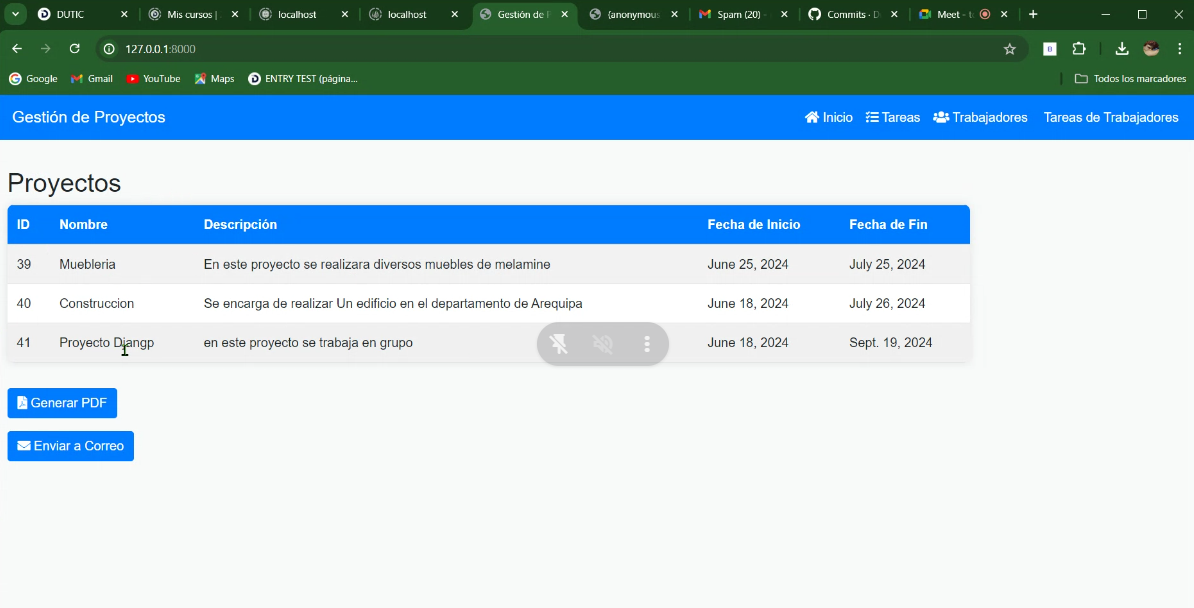
\includegraphics[width=0.9\textwidth]{img/principal.png}
    \caption{Página de los proyectos creados.}
\end{figure}

\begin{figure}[h]
    \centering
    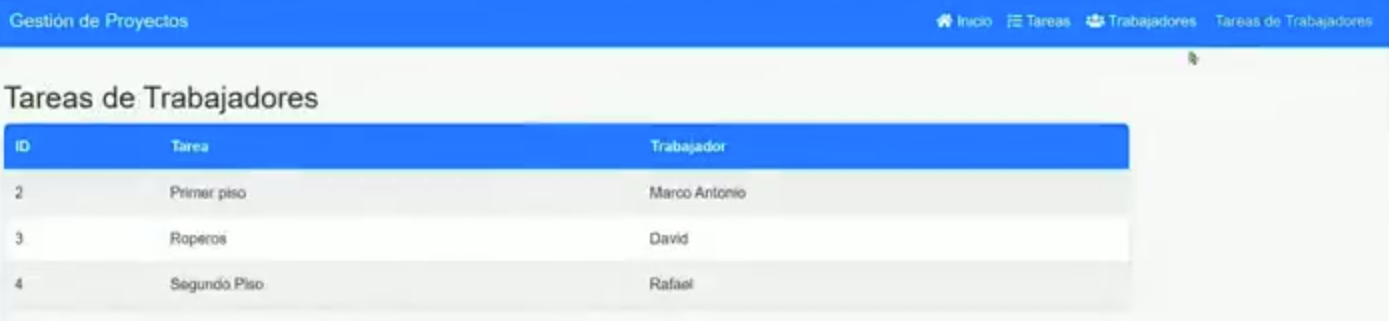
\includegraphics[width=0.9\textwidth]{img/template2.png}
    \caption{Página de las tareas.}
\end{figure}

\begin{figure}[h]
    \centering
    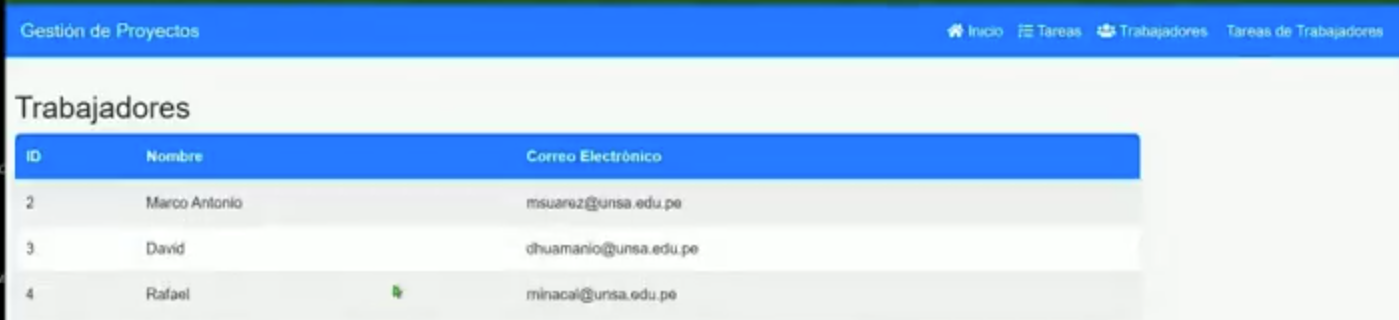
\includegraphics[width=0.9\textwidth]{img/template3.png}
    \caption{Página de los trabajadores creados.}
\end{figure}

\begin{figure}[h]
    \centering
    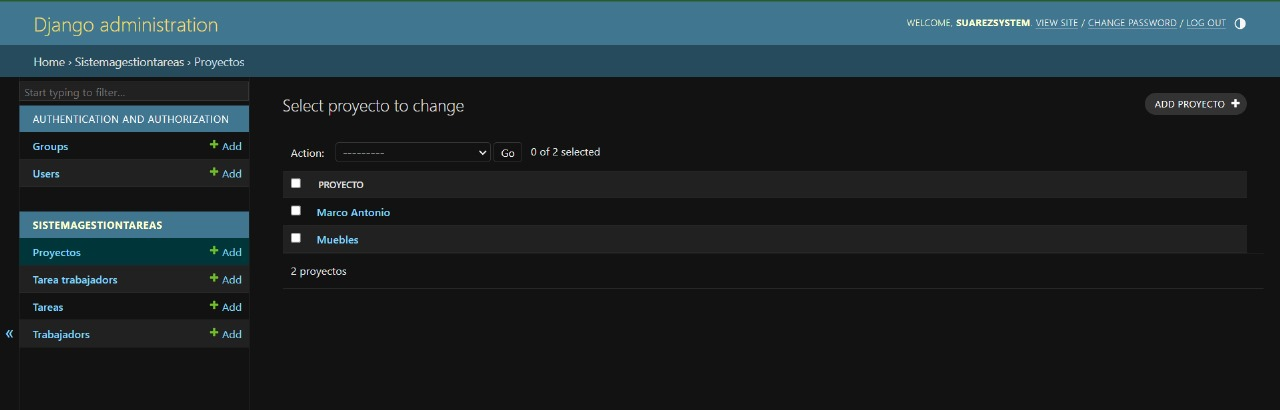
\includegraphics[width=0.9\textwidth]{img/template4.png}
    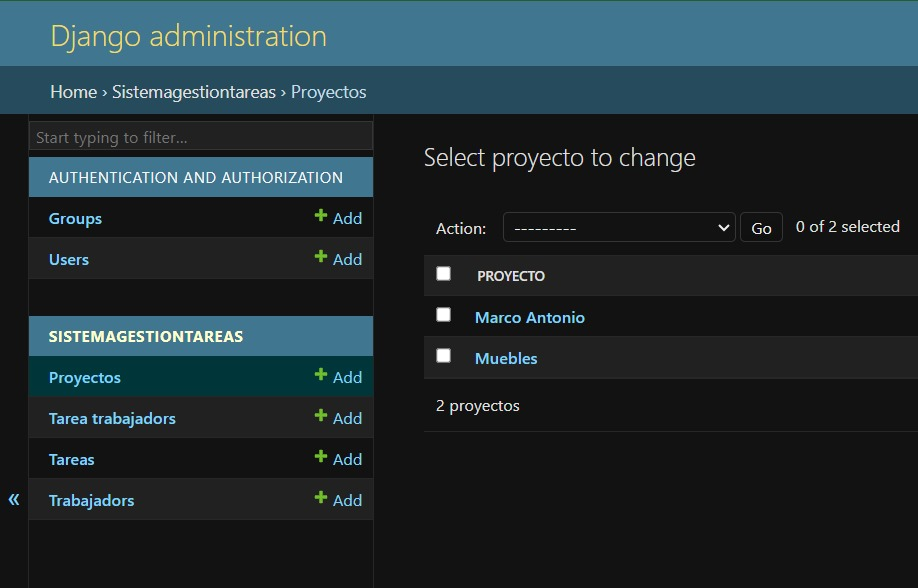
\includegraphics[width=0.9\textwidth]{img/template5.png}
    \caption{Página admin de las tablas creadas.}
\end{figure}

\begin{figure}[h]
    \centering
    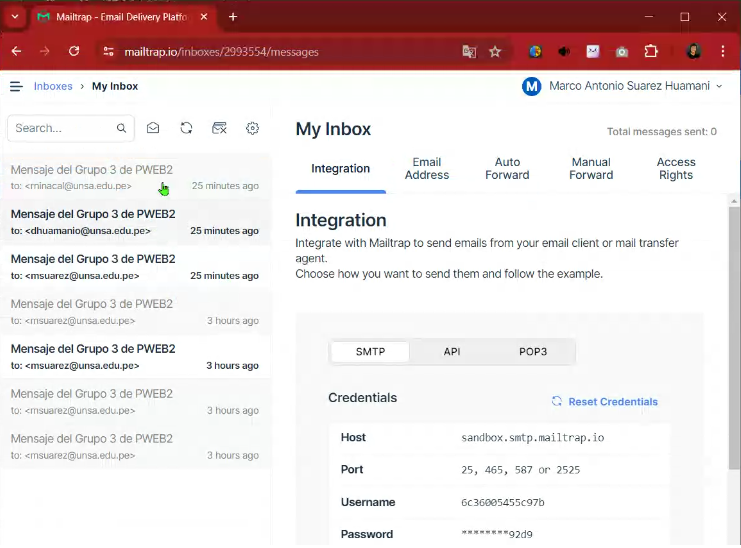
\includegraphics[width=0.9\textwidth]{img/correo.png}
    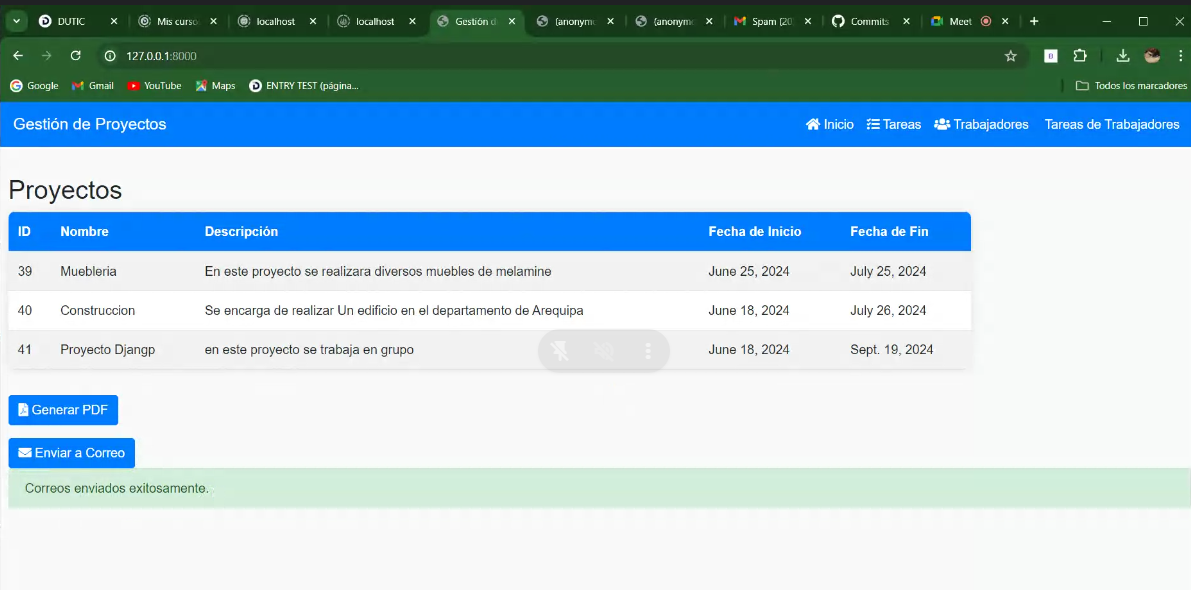
\includegraphics[width=0.9\textwidth]{img/correo1.png}
    \caption{Imagenes de los correos enviados}
\end{figure}

\begin{figure}[h]
    \centering
    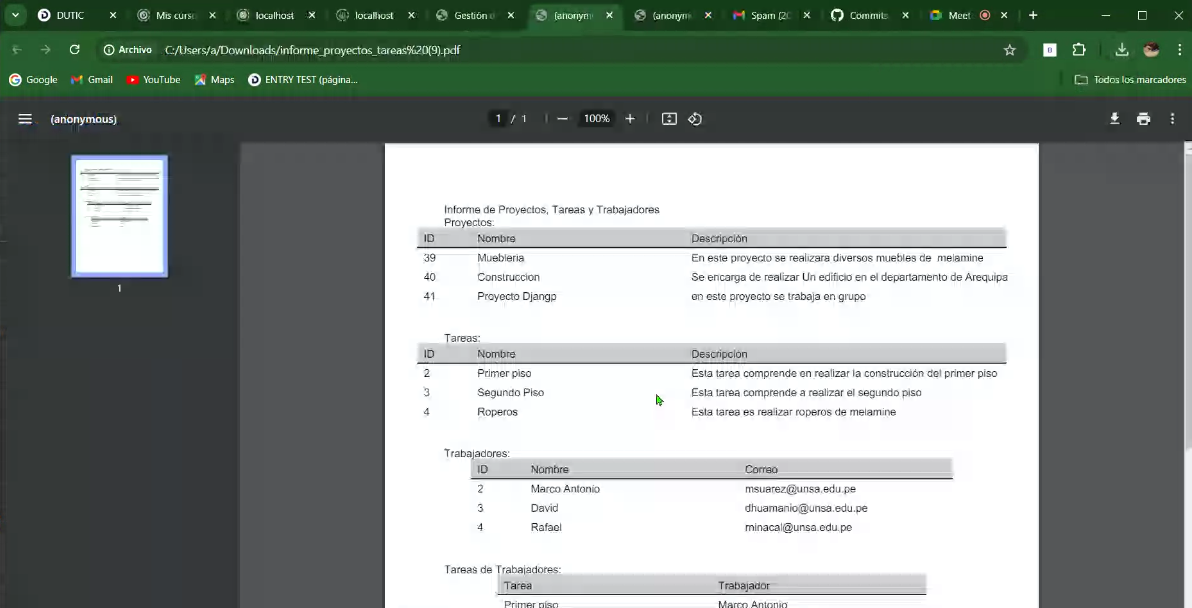
\includegraphics[width=0.9\textwidth]{img/pdf1.png}
    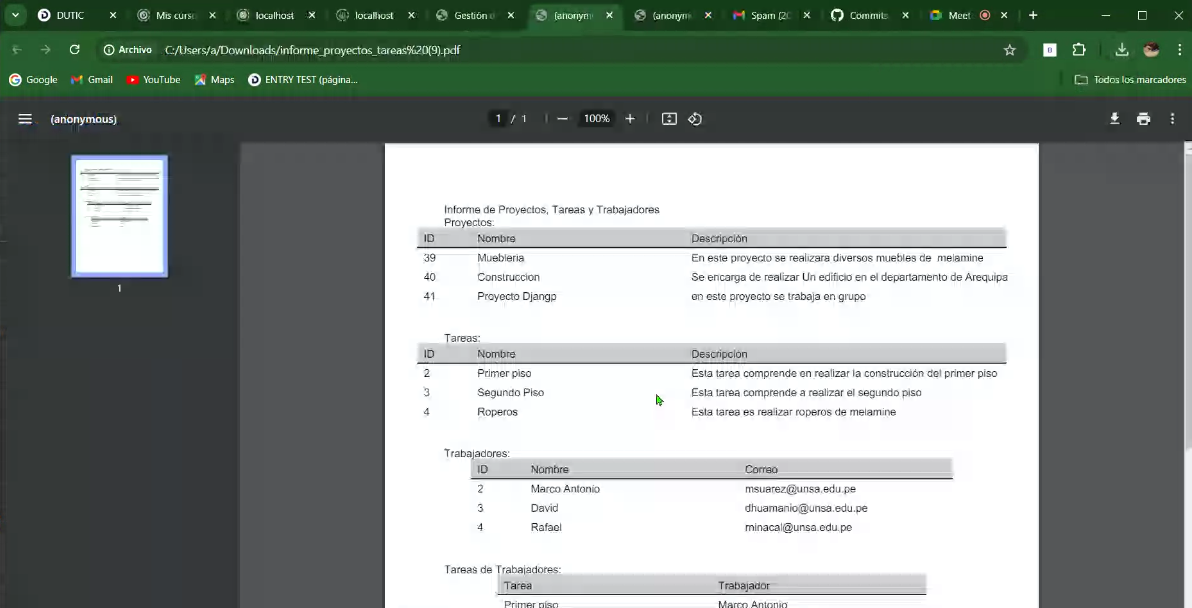
\includegraphics[width=0.9\textwidth]{img/pdf2.png}
    \caption{Imagenes del pdf generado.}
\end{figure}

\clearpage

 \section{Commits realizados}:

    \begin{lstlisting}[language=Python,caption={commits}][H]
* 893fcc5 (HEAD -> main, origin/main, origin/HEAD) Final del manage.py completo
* 88f6cdb funcionalidades completas , final
* 0a500f0 eliminación de credenciales de correo temporal
* d9dcd46 funcionalidades de enviar correo y generar pdf
* 3af2a73 Se quito las opciones de agregar y eliminar
* 2aa7418 Añadiendo latex y pdf
* f86e9db eliminando pdf
* b262f4c eliminando latex
* e3ee7f3 Add files via upload
* 2c46a13 proyecto culminado
* 4113a4d añadiendo el gestiontareas completado
* b7ab375 Delete Project_lab08 directory
* d267ccb Delete sistemagestiontareas
* 97c9907 actualizado el sistemagestiontareas
* 6695b81 todo settings.py actualizado
* cb39dbe añadiendo la base de datos
* 68fe603 Add files via upload
    \end{lstlisting}

\section{\textcolor{red}{Rúbricas}}
	
	\subsection{\textcolor{red}{Sobre el informe}}
	\begin{table}[H]
		\caption{Tipo de Informe}
		\setlength{\tabcolsep}{0.5em} % for the horizontal padding
		{\renewcommand{\arraystretch}{1.5}% for the vertical padding
		\begin{tabular}{|p{3cm}|p{12cm}|}
			\hline
			\multicolumn{2}{|c|}{\textbf{\textcolor{red}{Informe}}}  \\
			\hline 
			\textbf{\textcolor{red}{Latex}} & \textcolor{blue}{El informe está en formato PDF desde Latex,  con un formato limpio (buena presentación) y facil de leer.}   \\ 
			\hline 
			
			
		\end{tabular}
	}
	\end{table}


	\subsection{\textcolor{red}{Rúbrica para el contenido del Informe y demostración}}
	\begin{itemize}			
		\item El alumno debe marcar o dejar en blanco en celdas de la columna \textbf{Checklist} si cumplio con el ítem correspondiente.
		\item Si un alumno supera la fecha de entrega,  su calificación será sobre la nota mínima aprobada, siempre y cuando cumpla con todos lo items.
		\item El alumno debe autocalificarse en la columna \textbf{Estudiante} de acuerdo a la siguiente tabla:
	
		\begin{table}[ht]
			\caption{Niveles de desempeño}
			\begin{center}
			\begin{tabular}{ccccc}
    			\hline
    			 & \multicolumn{4}{c}{Nivel}\\
    			\cline{1-5}
    			\textbf{Puntos} & Insatisfactorio 25\%& En Proceso 50\% & Satisfactorio 75\% & Sobresaliente 100\%\\
    			\textbf{2.0}&0.5&1.0&1.5&2.0\\
    			\textbf{4.0}&1.0&2.0&3.0&4.0\\
    		\hline
			\end{tabular}
		\end{center}
	\end{table}	
	
	\end{itemize}
	
	\begin{table}[H]
		\caption{Rúbrica para contenido del Informe y demostración}
		\setlength{\tabcolsep}{0.5em} % for the horizontal padding
		{\renewcommand{\arraystretch}{1.5}% for the vertical padding
		%\begin{center}
		\begin{tabular}{|p{2.7cm}|p{7cm}|x{1.3cm}|p{1.2cm}|p{1.5cm}|p{1.1cm}|}
			\hline
    		\multicolumn{2}{|c|}{Contenido y demostración} & Puntos & Checklist & Estudiante & Profesor\\
			\hline
			\textbf{1. GitHub} & Hay enlace URL activo del directorio para el  laboratorio hacia su repositorio GitHub con código fuente terminado y fácil de revisar. &2 &X &2 & \\ 
			\hline
			\textbf{2. Commits} &  Hay capturas de pantalla de los commits más importantes con sus explicaciones detalladas. (El profesor puede preguntar para refrendar calificación). &4 &X &2 & \\ 
			\hline 
			\textbf{3. Código fuente} &  Hay porciones de código fuente importantes con numeración y explicaciones detalladas de sus funciones. &2 &X &2 & \\ 
			\hline 
			\textbf{4. Ejecución} & Se incluyen ejecuciones/pruebas del código fuente  explicadas gradualmente. &2 &X &2 & \\ 
			\hline			
			\textbf{5. Pregunta} & Se responde con completitud a la pregunta formulada en la tarea.  (El profesor puede preguntar para refrendar calificación).  &2 &X &2 & \\ 
			\hline	
			\textbf{6. Fechas} & Las fechas de modificación del código fuente estan dentro de los plazos de fecha de entrega establecidos. &2 &X &0.5 & \\ 
			\hline 
			\textbf{7. Ortografía} & El documento no muestra errores ortográficos. &2 &X &2 & \\ 
			\hline 
			\textbf{8. Madurez} & El Informe muestra de manera general una evolución de la madurez del código fuente,  explicaciones puntuales pero precisas y un acabado impecable.   (El profesor puede preguntar para refrendar calificación).  &4 &X &3 & \\ 
			\hline
			\multicolumn{2}{|c|}{\textbf{Total}} &20 & &15.5 & \\ 
			\hline
		\end{tabular}
		%\end{center}
		%\label{tab:multicol}
		}
	\end{table}
	
\clearpage

\section{Referencias}
\begin{itemize}			
	\item \url{https://docs.djangoproject.com/en/5.0/topics/db/examples/many\_to\_one/}
	\item \url{https://docs.djangoproject.com/}
	\item \url{https://www.w3schools.com/python/}
	\item \url{https://www.w3schools.com/django/}

\end{itemize}
\end{itemize}	
	
%\clearpage
%\bibliographystyle{apalike}
%\bibliographystyle{IEEEtranN}
%\bibliography{bibliography}
			
\end{document}
